\section{NOx onderzoek}
Stikstofoxides zijn verbindingen tussen stikstof en zuurstof in de vormen $NO$ en $NO_2$. Stikstofdioxide ($NO_2$) komt vrij bij de verbranding van fossielen brandstoffen. In Nederland zijn de grootste uitstoters van $NO_x$ het verkeer en de elektriciteitscentrales.  De uitstoot van $NO_2$ heeft gevolgen voor de natuur en de gezondheid. $NO_2$ word dan ook vaak gebruikt als indicator van de luchtkwaliteit.

\subsection{Effecten van NOx}
Stikstofoxide levert een bijdrage aan de vorming van zure regen. Blootstelling aan $NO_2$ hangt samen met luchtwegklachten zoals verminderende longfunctie, astma-aanvallen en infecties. $NO$ daarin tegen heeft weinig gezondheidseffecten \cite{NO2_Amsterdam}. 


\subsubsection{Normen}
De norm voor het jaargemiddelde $NO_2$ is 	$40\,\nicefrac{\mu g}{m^{3}}$. Deze norm wordt lokaal enkele keren per jaar overschreden. Omdat het verkeer veel $NO_2$ uitstoot, geld een maximaal toegestaan uurgemiddelde van $200\,\nicefrac{\mu g}{m^{3}}$ voor wegen waar meer dan 40.000 motorvoertuigen per etmaal gebruik van maken.

\begin{center}
	\begin{tabular}{ | m{5cm} | m{5cm}| } 
		\hline
		Soort norm & Concentratie \\
		\hline
		Jaargmiddelde & $40\,\nicefrac{\mu g}{m^{3}}$
		\\ 
		\hline
		Uurgemiddelde & $200\,\nicefrac{\mu g}{m^{3}}$* 
		\\ 
		\hline
	\end{tabular}
\end{center}

\begin{footnotesize} 
	* Van toepassing voor wegen waarvan ten minste 40.000 motorvoertuigen per etmaal gebruik maken.
\end{footnotesize}

De gemiddelde concentratie $NO_2$ in de Amsterdamse buitenlucht ligt rond de $25\,\nicefrac{\mu g}{m^{3}}$ (13 ppb). De concentraties binnen liggen meestal een factor 2 lager dan buiten. 

\begin{figure}
	\centering
	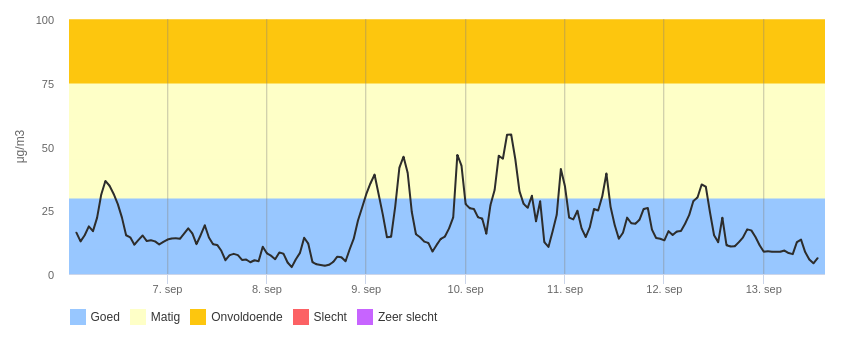
\includegraphics[width=.9\linewidth]{App1/media/amsterdam.png}
	\caption{Meetwaardes $NO_2$ Kantershof Amsterdam zuidoost. 6 tot 11 september 2019 \cite{grafiek}}
	\label{fig:grafiek}
\end{figure}

\newpage
\subsubsection{Sensoren}
Om de voorkomende niveau's te kunnen meten moet de gekozen sensor een meetbereik hebben tussen de 0 en de 40 ppb, met een resolutie van 1 ppb.\\
De NO2-B43F $NO_2$ sensor is een chemoresistive sensor van Alphasense en lijkt de beste optie maar is niet geschikt.\\
Deze sensor een meetbereik van 0 tot 20 ppm met een meetonzekerheid van 15 ppb. Deze sensor is niet gevoelig genoeg om de lage concentraties met een resolutie van 1 ppb uit de lucht goed te kunnen meten.\\ 
Sensoren die $NO_2$ meten hebben een kruisgevoeligheid voor andere gassen zoals $O_3$ en zijn erg gevoelig voor veranderingen in temperatuur en luchtvochtigheid. \\
De sensor moet energie zuinig zijn waardoor chemoresistive sensoren niet geschikt zijn omdat deze een continu verbruik is in de ordegrootte van 50 mW \cite{B4DF}. 

\subsubsection{Conclusie}
Er is geen sensor op de markt beschikbaar om de concentraties $NO_2$ die we verwachten te meten. De beschikbare sensoren zijn niet gevoelig genoeg en verbruiken te veel energie. Daarom is er voor gekozen om af te stappen van het meten van $NO_2$ als indicator van de luchtkwaliteit binnen de HvA gebouwen. Als alternatief is gekozen voor het meten van $CO$ concentraties in de lucht. $CO$ is een giftig gas en kan vrijkomen bij onvolledige verbrandingen en is daarom belangrijk om dit gas tijdig te registreren.